%%%%%%%%%%%%%%%%%%%%%%%%%%%%%%%%%%%%%%%%%%%%%%%%%%%%%%%%%%%
\subsection{Apply statistical model to data}
%%%%%%%%%%%%%%%%%%%%%%%%%%%%%%%%%%%%%%%%%%%%%%%%%%%%%%%%%%%
%
%
\begin{frame}[t, negative]
	\subsectionpage
\end{frame}
%
%
\begin{lhframe}[rhgraphic={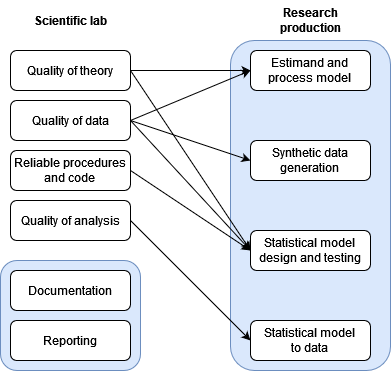
\includegraphics[scale=0.43]{lab_to_research.png}}]
	{What we have so far}
	
	\begin{enumerate}
		%
		\item measure: \\
		{\small replicated entropies $H^{O}_{ik}$ }
		%
		\item estimand: \\
		{\small $SI$ index, structural parameters, contrasts }
		%
		\item structural models: \\
		{\small total and direct effects }
		%
		\item probabilistic models: \\
		{\small three possible fitting models }
		%
		\item statistical models: \\
		{\small works as intended }
		%
		\item power: \\
		{\small enough }
		%
	\end{enumerate} 
	%
\end{lhframe}
%
%
\begin{lhframe}[rhgraphic={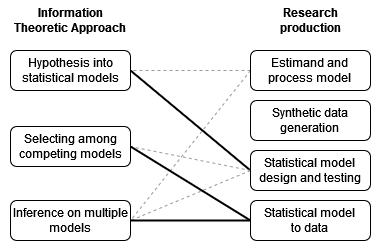
\includegraphics[scale=0.63]{ITA_to_research.png}}]
	{Information Theoretic Approach \cite{Anderson_2008, Chamberlain_1965} }
	
	The last step would be \textcolor{blue}{select the most fitting model} using the ITA,
	\begin{enumerate}
		%
		\item \sout{hypothesis into statistical models},
		\item select among competing models, 
		\item make inferences based on one or multiple models.
		%
	\end{enumerate}
	%
	the most fitting model based on information criteria,
	\begin{itemize}
		%
		\item WAIC \cite{Watanabe_2013}
		\item PSIS \cite{Vehtari_et_al_2021}
		%
	\end{itemize}
	%
\end{lhframe}
%
%
\begin{frame}
	{Revisiting our theory}
	%
	\begin{columns}
		%
		\begin{column}{0.5\textwidth}
			%
			\begin{itemize}
				%
				\item $H_{ik}=$ (observed) entropy replicates
				%
				\item $H_{i}=$ (latent) ``true" entropy
				%
				\item $SI_{i}=$ (latent) SI score \\
				{\small \textcolor{blue}{(inversely related to $H^{T}_{i}$)} }
				%
				\item $A_{i}=$ ``hearing" age (minimum)
				%
				\item $E_{i}=$ etiology of disease
				%
				\item $HS_{i}=$ hearing status
				%
				\item $PTA_{i}=$ pure tone average (standardized)
				%
				\item $B_{bk}=$ block {\small \textcolor{blue}{(will reduce $\sigma_{U_{ik}}$) } }
				%
				\item variables \textcolor{blue}{assumed independent}, beyond the described relationships,
				\begin{equation*}
					%
					\begin{aligned} 
						P(\pmb{U}) & = P(U_{ik}, U_{i}, U_{A}, U_{E}, U_{HS}, U_{P}, B_{bk}) \\ 
						& = P(U_{ik}) P(U_{i}) P(U_{A}) P(U_{E}) P(U_{HS}) P(U_{P}) P(B_{bk})
					\end{aligned}
					%
				\end{equation*}
				%
			\end{itemize}
			%
		\end{column}
		%
		\begin{column}{0.5\textwidth}  
			%
			\begin{figure}
				%
				\begin{tikzpicture}
					% nodes
					\node at (3,0) {$H^{O}_{ik}$};
					\node at (2,-0.7) {$U_{ik}$};
					\node at (1,-0.4) {$H^{T}_{i}$};
					\node at (-0.5,-0.4) {$SI_{i}$};
					\node at (-1.5,-0.7) {$U_{i}$};
					\node at (-0.9,1.75) {$HS_{i}$};
					\node at (-0.5,2.7) {$U_{HS}$};
					\node at (-2.2,1.5) {$E_{i}$};
					\node at (-2,2.7) {$U_{E}$};
					\node at (1.5,1.5) {$PTA_{i}$};
					\node at (1,2.7) {$U_{P}$};
					\node at (-2.1,1) {$A_{i}$};
					\node at (-2.8,1) {$U_{A}$};
					\node at (2,0.7) {$B_{bk}$};
					
					% paths
					\draw[{Circle[open]}-{latex}](0.85,0)--(2.6,0); % Hi->Hik
					\draw[{Circle[open]}-{latex}{Circle}](1.9,-0.4)--(2.7,0); % Uik->Hik
					\draw[{Circle[open]}-{latex}](1.9,0.4)--(2.6,0.05); % Bi->SIi
					\draw[{Circle[open]}-{latex}](-0.5,0)--(0.85,0); % SIi->Hi
					\draw[{Circle[open]}-{latex}](-1.6,-0.4)--(-0.5,0); % Ui->SIi
					\draw[{Circle}-{latex}](-0.45,1.6)--(-0.45,0.05); % HSi->SIi
					\draw[-{latex}](-0.45,1.50)--(-1.90,0.75); % HSi->Ai
					\draw[-{latex}](-0.45,1.5)--(0.9,1.5); % HSi->PTAi
					\draw[{Circle}-{latex}](-2,1.5)--(-0.5,1.5); % Ei->HSi
					\draw[-{latex}](-1.9,1.45)--(-0.47,0.05); % Ei->SIi
					\draw[{Circle}-{latex}](0.95,1.55)--(-0.4,0.05); % PTAi->SIi
					\draw[{Circle}-{latex}](-2,0.75)--(-0.5,0); % Ai->SIi
					\draw[{Circle[open]}-{latex}](-1.95,2.5)--(-1.95,1.6); % UE->Ei
					\draw[{Circle[open]}-{latex}](-0.45,2.5)--(-0.45,1.6); % UHS->HSi
					\draw[{Circle[open]}-{latex}](0.95,2.5)--(0.95,1.6); % UP->PTAi
					\draw[{Circle[open]}-{latex}](-2.8,0.70)--(-2,0.70); % UA->Ai
					
					% extras
					\node at (0.2,-0.25) {$(-)$}; % symbol
					\draw[dotted, thick] (1.5,1) rectangle (3.5,-1);
					%\node at (2,0.7) {$k=1,\dots,K$};
					\draw[dashed] (-3.2,3) rectangle (3.7,-1.2);
					%\node at (2,0.7) {$k=1,\dots,K$};
				\end{tikzpicture}
				%
				\caption*{General structural diagram}
			\end{figure}
			%
		\end{column}
		%
	\end{columns}
	%
\end{frame}
%
%
\begin{frame}
	{Interested in two effects}
	%
	\begin{columns}
		%
		\begin{column}{0.5\textwidth}
			%
			\begin{enumerate}
				%
				\item \textcolor{blue}{total effects} model inherits:
				%
				\begin{itemize}
					%
					\item children’s characteristics that lead to the fitting of specific apparatus,
					%
					\item the (convenience of) sample selection \textcolor{blue}{(fixed with post-stratification)}
					%
				\end{itemize}
				%
				\item to do the last, we stratify for all variables that explain variability, ergo, use a \textcolor{blue}{direct effects} model
				%
				\item \underline{three levels:} \\
				replicates ($k$), children ($i$), blocks ($b$), \\
				{\small \textcolor{blue}{(denoted by discontinuous squares)}}
				%
			\end{enumerate}
			%
		\end{column}
		%
		\begin{column}{0.5\textwidth}  
			%
			\begin{figure}
				%
				\begin{tikzpicture}
					% nodes
					\node at (3,0) {$H^{O}_{ik}$};
					\node at (2,-0.7) {$U_{ik}$};
					\node at (1,-0.4) {$H^{T}_{i}$};
					\node at (-0.5,-0.4) {$SI_{i}$};
					\node at (-1.5,-0.7) {$U_{i}$};
					\node at (-0.9,1.2) {$HS_{i}$};
					%\node at (-0.5,2.7) {$U_{HS}$};
					\node at (-2.2,1) {$E_{i}$};
					%\node at (-2,2.7) {$U_{E}$};
					%\node at (1.5,1.5) {$PTA_{i}$};
					%\node at (1,2.7) {$U_{P}$};
					%\node at (-2,1) {$A_{i}$};
					%\node at (-2.8,1) {$U_{A}$};
					\node at (2,0.7) {$B_{bk}$};
					
					% paths
					\draw[{Circle[open]}-{latex}](0.85,0)--(2.6,0); % Hi->Hik
					\draw[{Circle[open]}-{latex}{Circle}](1.9,-0.4)--(2.7,0); % Uik->Hik
					\draw[{Circle[open]}-{latex}](1.9,0.4)--(2.6,0.05); % Bi->SIi
					\draw[{Circle[open]}-{latex}](-0.5,0)--(0.85,0); % SIi->Hi
					\draw[{Circle[open]}-{latex}](-1.6,-0.4)--(-0.5,0); % Ui->SIi
					\draw[{Circle}-{latex}](-0.45,1.05)--(-0.45,0.05); % HSi->SIi
					%\draw[-{latex}](-0.45,0.95)--(-1.90,0.75); % HSi->Ai
					\draw[{Circle}-{latex}](-2,1)--(-0.5,1); % Ei->HSi
					\draw[-{latex}](-1.9,1)--(-0.47,0.05); % Ei->SIi
					%\draw[{Circle}-{latex}](1,1.5)--(-0.4,1.5); % PTAi->HSi
					%\draw[-{latex}](0.9,1.45)--(-0.4,0.05); % PTAi->SIi
					%\draw[{Circle}-{latex}](-2,0.75)--(-0.5,0); % Ai->SIi
					%\draw[{Circle[open]}-{latex}](-1.95,2.5)--(-1.95,1.6); % UE->Ei
					%\draw[{Circle[open]}-{latex}](-0.45,2.5)--(-0.45,1.6); % UHS->HSi
					%\draw[{Circle[open]}-{latex}](0.95,2.5)--(0.95,1.6); % UP->PTAi
					%\draw[{Circle[open]}-{latex}](-2.8,0.70)--(-2,0.70); % UA->Ai
					
					% extras
					\node at (0.2,-0.25) {$(-)$}; % symbol
					\draw[dotted, thick] (1.5,1) rectangle (3.5,-1);
					%\node at (2,0.7) {$k=1,\dots,K$};
					\draw[dashed] (-2.5,1.45) rectangle (3.7,-1.2);
					%\node at (2,0.7) {$k=1,\dots,K$};
				\end{tikzpicture}
				\caption*{(b) total effects}
			\end{figure}
			%
			\begin{figure}
				%
				\begin{tikzpicture}
					% nodes
					\node at (3,0) {$H^{O}_{ik}$};
					\node at (2,-0.7) {$U_{ik}$};
					\node at (1,-0.4) {$H^{T}_{i}$};
					\node at (-0.5,-0.4) {$SI_{i}$};
					\node at (-1.5,-0.7) {$U_{i}$};
					\node at (-0.9,1.75) {$HS_{i}$};
					%\node at (-0.5,2.7) {$U_{HS}$};
					\node at (-2.2,1.5) {$E_{i}$};
					%\node at (-2,2.7) {$U_{E}$};
					\node at (1.5,1.5) {$PTA_{i}$};
					%\node at (1,2.7) {$U_{P}$};
					\node at (-2.1,1) {$A_{i}$};
					%\node at (-2.8,1) {$U_{A}$};
					\node at (2,0.7) {$B_{bk}$};
					
					% paths
					\draw[{Circle[open]}-{latex}](0.85,0)--(2.6,0); % Hi->Hik
					\draw[{Circle[open]}-{latex}{Circle}](1.9,-0.4)--(2.7,0); % Uik->Hik
					\draw[{Circle[open]}-{latex}](1.9,0.4)--(2.6,0.05); % Bi->SIi
					\draw[{Circle[open]}-{latex}](-0.5,0)--(0.85,0); % SIi->Hi
					\draw[{Circle[open]}-{latex}](-1.6,-0.4)--(-0.5,0); % Ui->SIi
					\draw[{Circle}-{latex}](-0.45,1.6)--(-0.45,0.05); % HSi->SIi
					\draw[-{latex}](-0.45,1.50)--(-1.90,0.75); % HSi->Ai
					\draw[-{latex}](-0.45,1.5)--(0.9,1.5); % HSi->PTAi
					\draw[{Circle}-{latex}](-2,1.5)--(-0.5,1.5); % Ei->HSi
					\draw[-{latex}](-1.9,1.45)--(-0.47,0.05); % Ei->SIi
					\draw[{Circle[color=red]}-{latex}](0.95,1.55)--(-0.4,0.05); % PTAi->SIi
					\draw[{Circle[color=red]}-{latex}](-2,0.75)--(-0.5,0); % Ai->SIi
					%\draw[{Circle[open]}-{latex}](-1.95,2.5)--(-1.95,1.6); % UE->Ei
					%\draw[{Circle[open]}-{latex}](-0.45,2.5)--(-0.45,1.6); % UHS->HSi
					%\draw[{Circle[open]}-{latex}](0.95,2.5)--(0.95,1.6); % UP->PTAi
					%\draw[{Circle[open]}-{latex}](-2.8,0.70)--(-2,0.70); % UA->Ai
					
					% extras
					\node at (0.2,-0.25) {$(-)$}; % symbol
					\draw[dotted, thick] (1.5,1) rectangle (3.5,-1);
					%\node at (2,0.7) {$k=1,\dots,K$};
					\draw[dashed] (-2.5,2) rectangle (3.7,-1.2);
					%\node at (2,0.7) {$k=1,\dots,K$};
				\end{tikzpicture}
				\caption*{(a) direct effects}
			\end{figure}
			%
		\end{column}
		%
	\end{columns}
	%
\end{frame}
%
%
\begin{lhframe}[rhgraphic={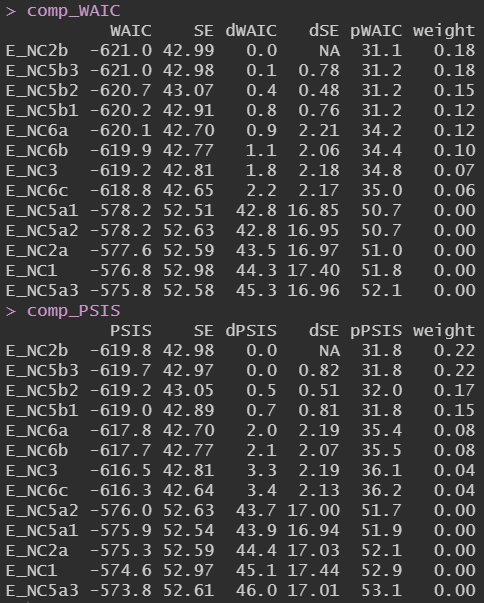
\includegraphics[scale=0.59]{models_table.png}}]
	{Competing models}
	
	We can notice,
	%
	\begin{itemize}
		%
		\item \textcolor{blue}{No evidence} in favor of models with $M=10$, i.e. $\text{weight}=0$ \\
		\underline{models:} \texttt{E\_NC1}, \texttt{E\_NC2a}, \texttt{E\_NC5a1}, \texttt{E\_NC5a2}, \texttt{E\_NC5a3}. 
		%
		\item \textcolor{blue}{Less evidence} in favor of ``robust" models, i.e. one $M$ per child \\
		\underline{models:} \texttt{E\_NC6a}, \texttt{E\_NC6b}, \texttt{E\_NC6c}. 
		%
		\item \textcolor{blue}{Mild evidence} in favor of ``robust" model without interaction \\
		\underline{models:} \texttt{E\_NC3}. \\
		{\small (qualifies as ME the lack of explanation at the child level)} \\
		%
	\end{itemize}
	%
\end{lhframe}
%
%
\begin{lhframe}[rhgraphic={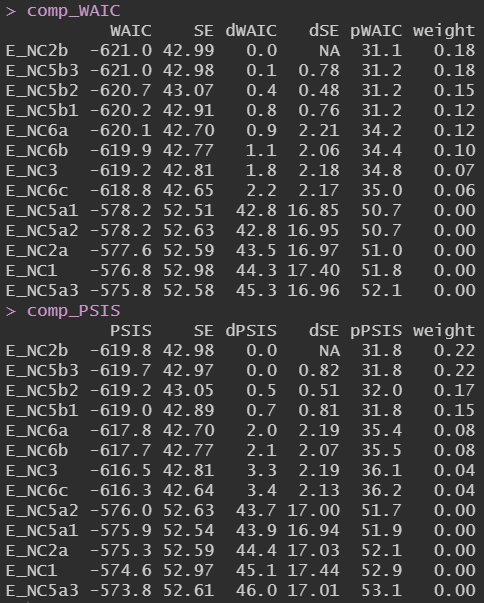
\includegraphics[scale=0.59]{models_table.png}}]
	{Competing models}
	
	further,
	%
	\begin{itemize}
		%
		\item \textcolor{blue}{Highest evidence} in favor of ``simplest" model, i.e. one $M$, no interaction \\ 
		\underline{models:} \texttt{E\_NC2b}.
		%
		\item However, interaction models are \textcolor{blue}{indistinguishable} from the ``simplest" model \\
		\underline{models:} \texttt{E\_NC5b1}, \texttt{E\_NC5b2}, \texttt{E\_NC5b3}.
		%
	\end{itemize}
	%
\end{lhframe}
%
%
\begin{lhframe}[rhgraphic={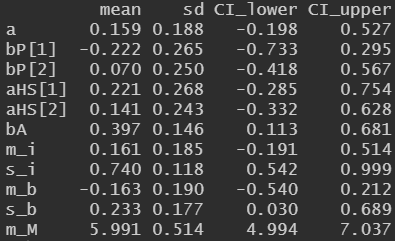
\includegraphics[scale=0.70]{select_model1.png}}]
	{Selecting models}
	
	``simplest" model (\texttt{E\_NC2b}) provides (preliminar) evidence on,
	%
	\begin{itemize}
		%
		\item the higher the unaided $PTA$ the lower the child's $SI$ ($bP[2]$)\\
		{\small (based on power analysis, \textcolor{blue}{we can be sure} is a small effect) }
		%
		\item no statistical difference between $NH$ and $HI/CI$ children \\
		{\small (but this requires a \textcolor{blue}{contrast}) }
		%
		\item for each ``hearing" year the $SI$ increases in $\approx 0.40$ logits \\
		{\small (\textcolor{blue}{larger than expected} effect assumed in power analysis) }
		%
	\end{itemize}
	%
\end{lhframe}
%
%
\begin{lhframe}[rhgraphic={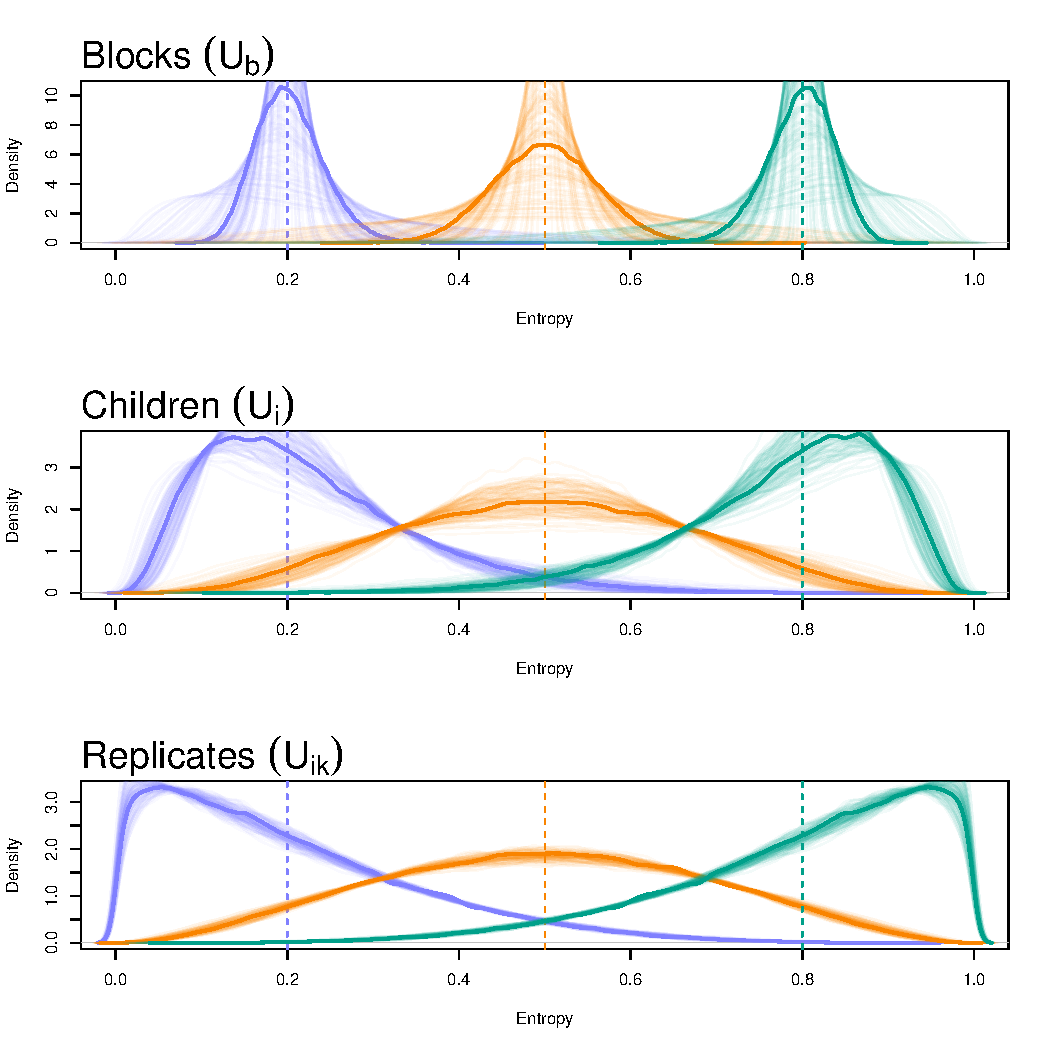
\includegraphics[scale=0.36]{variability_plot.pdf}}]
	{Selecting models}
	
	in addition in the ``simplest" model,
	%
	\begin{itemize}
		%
		\item it is hard to determine how the variability is ``explained" just by looking at the parameters \texttt{s\_b}, \texttt{s\_i}, \texttt{m\_M}
		%
		\item transforming the parameters into $[0,1]$ entropy scale:
		%
		\begin{itemize}
			\item block level (\texttt{s\_b}) has the lowest variability,
			%
			\item the individual level (\texttt{s\_i}) follows,
			%
			\item the measurement level variability (\texttt{m\_M}) has the highest
		\end{itemize}
		%
	\end{itemize}
	%
\end{lhframe}
%
%
\begin{lhframe}[rhgraphic={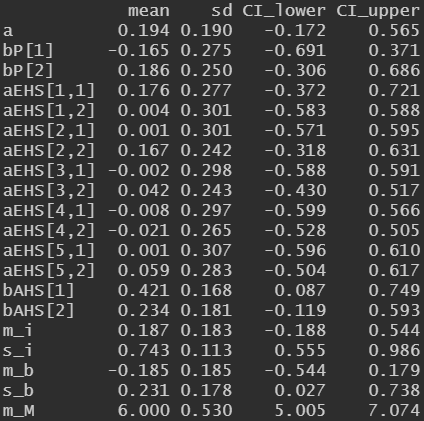
\includegraphics[scale=0.65]{select_model2.png}}]
	{Selecting models}
	
	however, the ``interaction" model (\texttt{E\_NC5b3}) provides evidence on,
	%
	\begin{itemize}
		%
		\item effects of the unaided $PTA$ on the child's $SI$ still non-significant
		%
		\item similar explained variability across levels and blocks \\
		{\small \textcolor{blue}{(similar to the ``simplest" model)}}
		%
		\item but ``mild" evidence of prevalent interactions,
		%
		\begin{itemize}
			\item $SI$ means for $HI/CI$ per $E$, \\
			$aEHS[2,2]$ (CMV) vs \\
			$aEHS[3,2]$ (Connexine 26)
			%
			\item different $SI$ evolution per unit $A$ ($bAHS$), $NH$ vs $HI/CI$ children
		\end{itemize}
		%
	\end{itemize}
	%
\end{lhframe}
%
%
\begin{lhframe}[rhgraphic={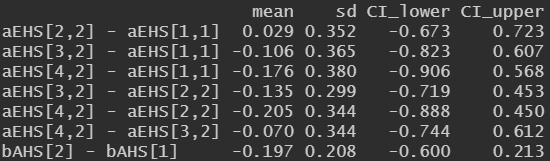
\includegraphics[scale=0.50]{contrasts.png}}]
	{Selecting models}
	
	within the ``interaction" model,
	%
	\begin{itemize}
		%
		\item the \textcolor{blue}{size of the data within groups} from combinations of $E$ and $HS$, does not allow to reject the contrasts' null hypothesis,
		%
		\item similar result is observed on the $bAHS$ contrast \\
		{\small (because the effect is small, compared to children's variability)}
		%
		\item still we decide to \textcolor{blue}{keep} the \textcolor{blue}{(\texttt{E\_NC5b3})} model 
		%
	\end{itemize}
	%
\end{lhframe}
%
%
\begin{lhframe}[rhgraphic={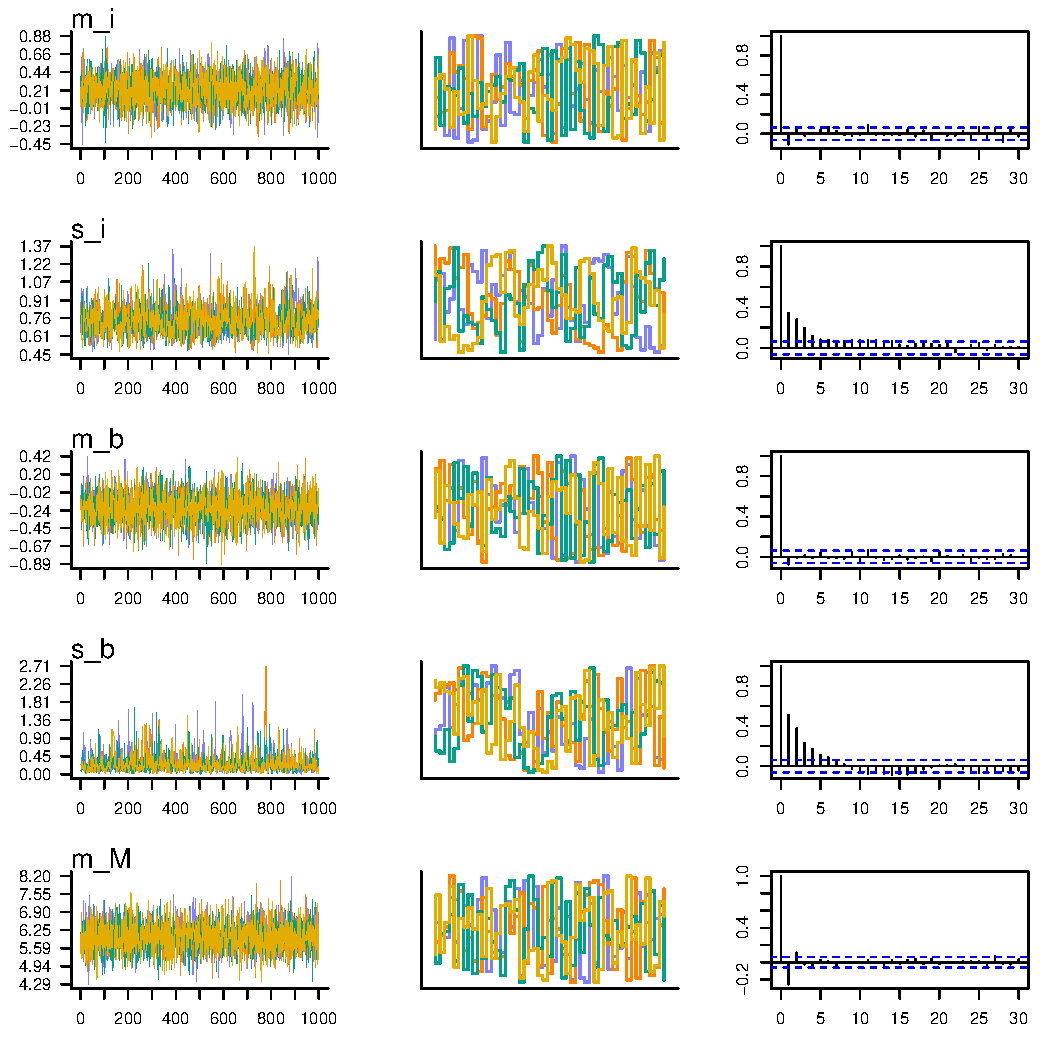
\includegraphics[scale=0.40]{chains_real1.pdf}}]
	{``Health" of MCMC chains}
	
	The MCMC chains achieve,
	%
	\begin{itemize}
		%
		\item good convergence
		\item good mixing
		\item lack of autocorrelation
		%
	\end{itemize}
	
	same results on the \textcolor{blue}{ \texttt{n\_eff} } and \textcolor{blue}{ \texttt{RHat} } statistics.
	%
\end{lhframe}
%
%
\begin{lhframe}[rhgraphic={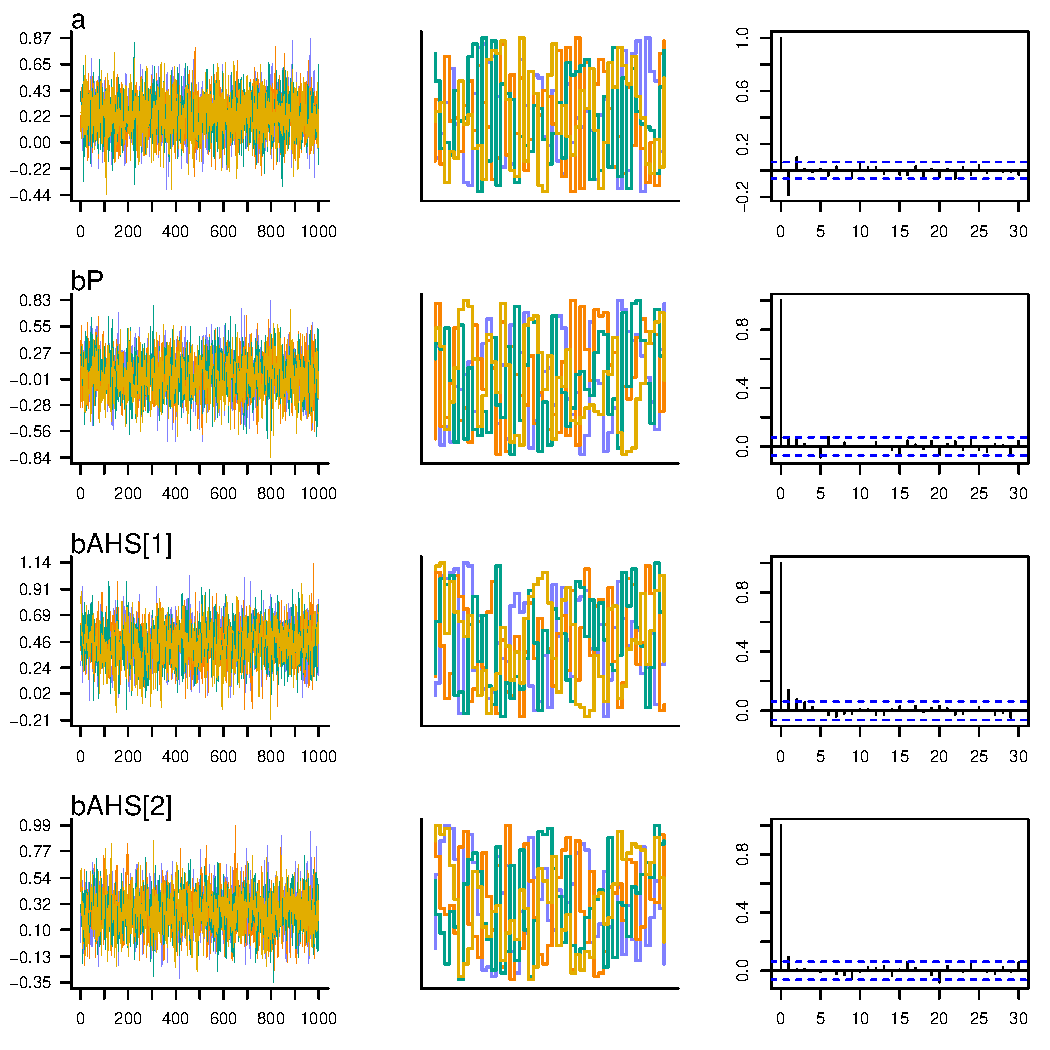
\includegraphics[scale=0.40]{chains_real2.pdf}}]
	{``Health" of MCMC chains}
	
	The MCMC chains achieve,
	%
	\begin{itemize}
		%
		\item good convergence
		\item good mixing
		\item lack of autocorrelation
		%
	\end{itemize}
	
	same results on the \textcolor{blue}{ \texttt{n\_eff} } and \textcolor{blue}{ \texttt{RHat} } statistics.
	%
\end{lhframe}
%
%
\begin{lhframe}[rhgraphic={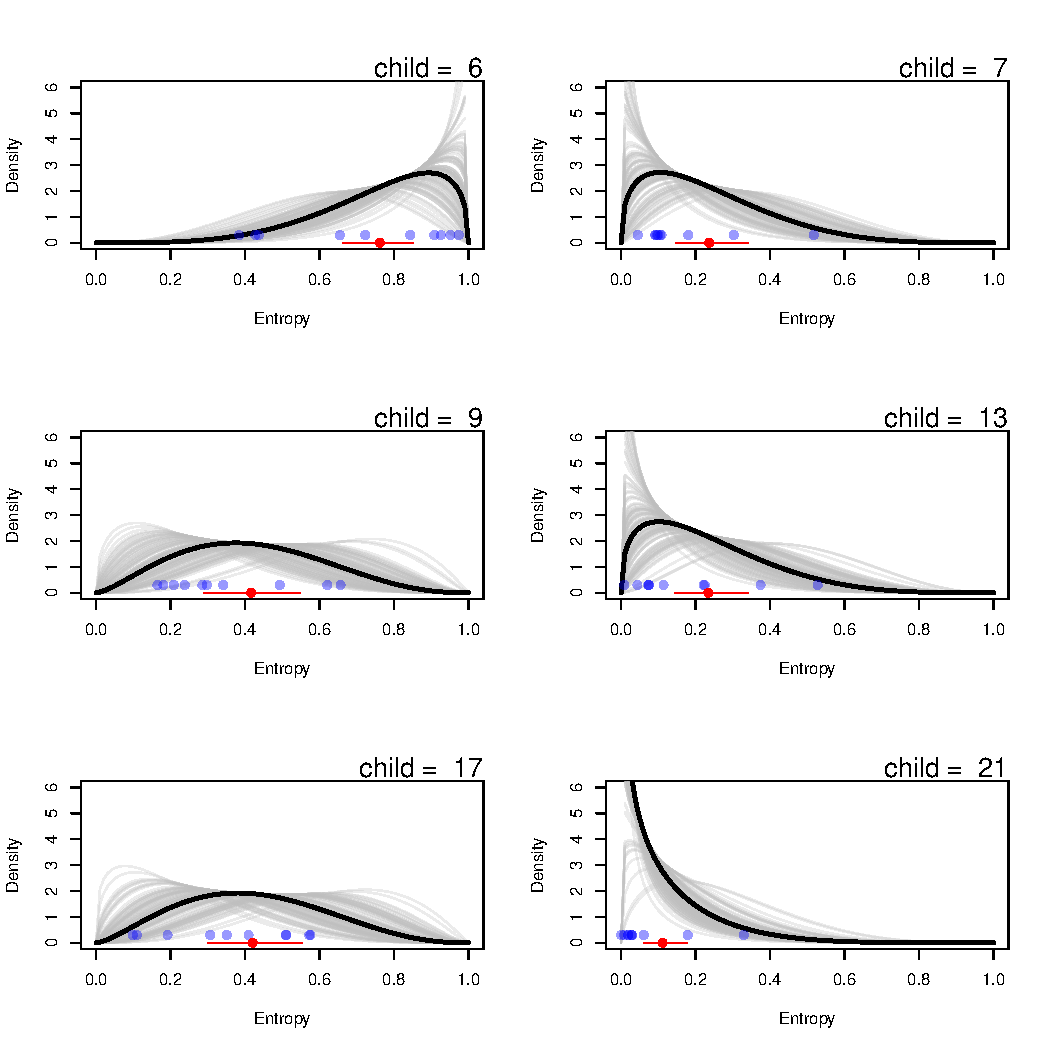
\includegraphics[scale=0.36]{posterior_predictive_real.pdf}}]
	{Posterior predictive}
	
	But how well reproduces the data?,
	%
	\begin{itemize}
		%
		\item captures the variability of the replicates,
		\item provides a ``true" $H$ (entropy) and $SI$ measures
		\item we can also make contrast of $SI$ measures per child
		%
	\end{itemize}
	%
\end{lhframe}
%
%
\begin{lhframe}[rhgraphic={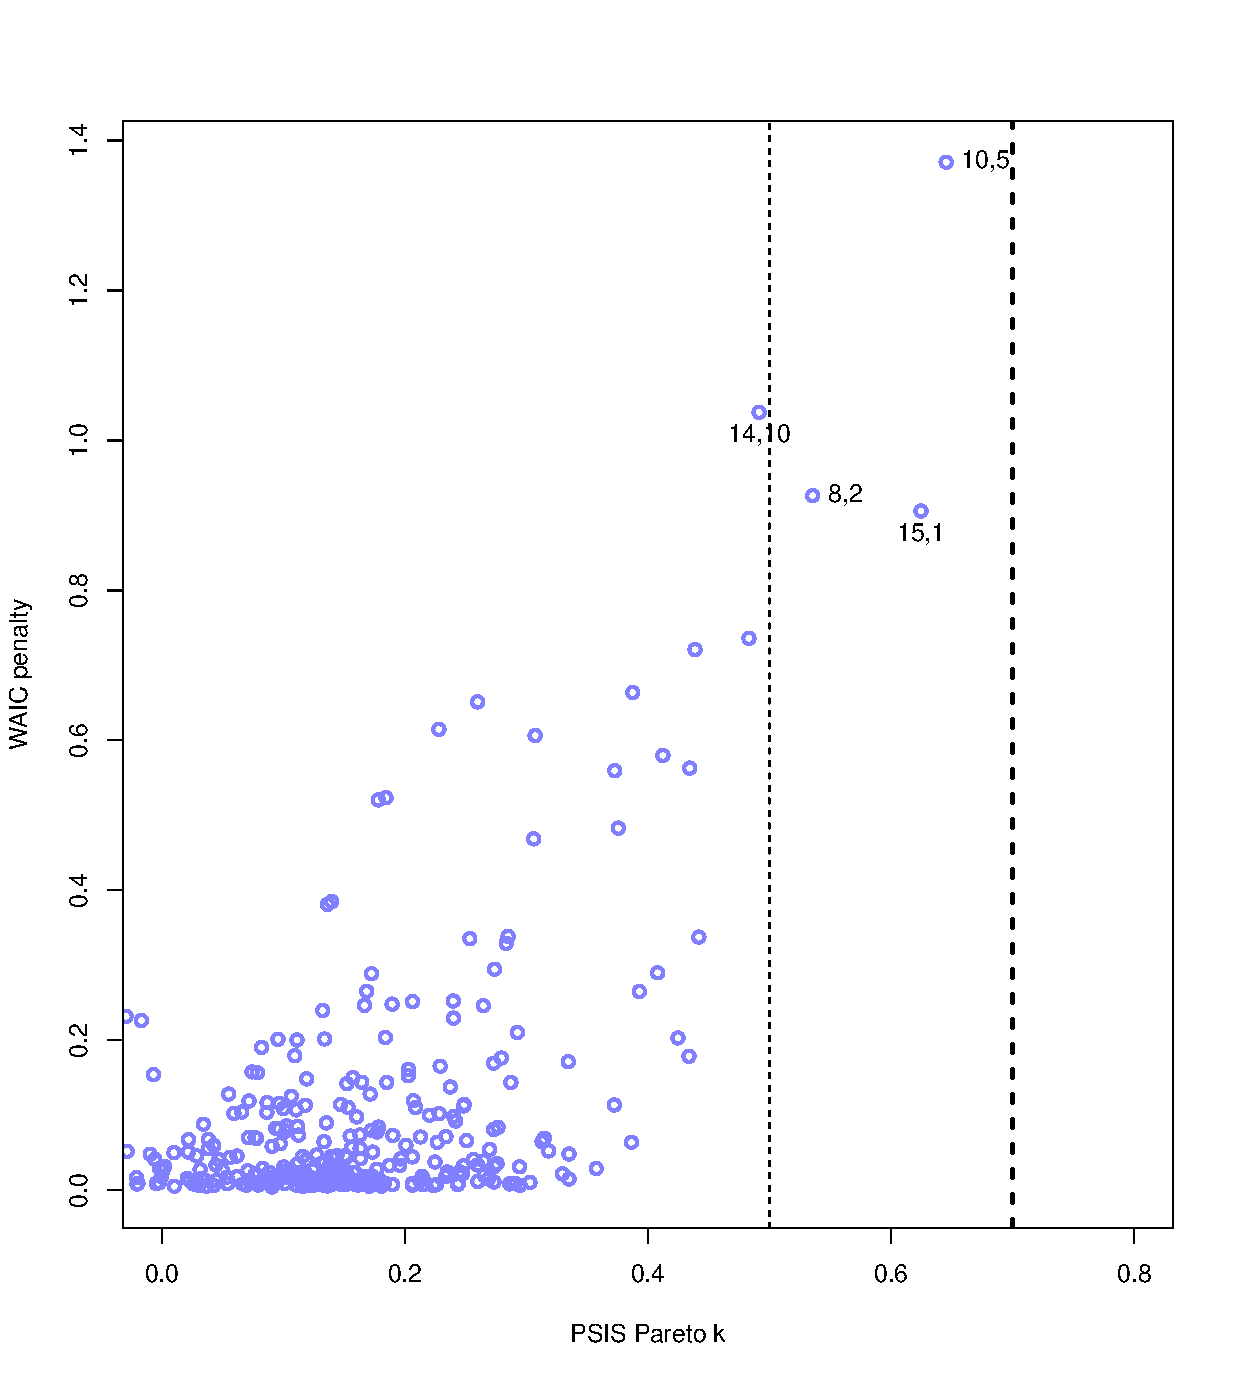
\includegraphics[scale=0.36]{outliers.pdf}}]
	{High leverage observations}
	
	``interaction" model has five (5) ``high" leverage observations, \\
	{\small \textcolor{blue}{(observations that ``drag" the estimation)} }
	%
	\begin{itemize}
		%
		\item the ``drag" is not large ($k<0.7$),
		%
		\item pair \textcolor{blue}{$(child, utterance)$} reveals,
		%
		\begin{itemize}
			%
			\item all cases cases have $H_{ik}=0$ \\
			{\small (next minimum value is $\approx 0.01$)}
			%
			\item child $25$ is $HI/CI$, with $A \approx 6.17$, \\
			{\small (the youngest $HI/CI$ child with ``perfect" $H_{ik}$, the utterance is a well developed word, for him/her?)}
			%
			\item no other relationship among them
			%
		\end{itemize}
		%
	\end{itemize}
	%
\end{lhframe}
%
%
